\documentclass[dvipdfmx,11pt,notheorems]{beamer}
%%%% 和文用 %%%%%
\usepackage{bxdpx-beamer}
\usepackage{pxjahyper}
\usepackage{minijs}%和文用
\usepackage{listings,jlisting} % プログラムの表示用
\usepackage{type1cm}
\renewcommand{\kanjifamilydefault}{\gtdefault}%和文用

%%%% スライドの見た目 %%%%%
\usetheme{Boadilla}
\usecolortheme{seahorse}
\usefonttheme{professionalfonts}
\setbeamertemplate{frametitle}[default][center]
\setbeamertemplate{navigation symbols}{}
\setbeamercovered{transparent}%好みに応じてどうぞ)
\setbeamertemplate{footline}[page number]
\setbeamerfont{footline}{size=\normalsize,series=\bfseries}
\setbeamercolor{footline}{fg=black,bg=black}

\setbeamercolor{white-cyan1}
{fg=white,bg=cyan!80!black}
\setbeamercolor{white-cyan2}
{fg=white,bg=cyan!60!black}

%フラットデザイン化
\setbeamertemplate{blocks}[rounded] % Blockの影を消す
%Beamer色設定
\definecolor{UniBlue}{RGB}{0,150,200}
\definecolor{AlertOrange}{RGB}{255,76,0}
\definecolor{AlmostBlack}{RGB}{38,38,38}
\setbeamercolor{structure}{fg=UniBlue} % 見出しカラー
\setbeamercolor{block title}{fg=UniBlue!50!black} % ブロック部分タイトルカラー
%%%%

%%%% 定義環境 %%%%%
\usepackage{amsmath,amssymb}
\usepackage{amsthm}
\usepackage{bm}
\theoremstyle{definition}
\newtheorem{theorem}{定理}
\newtheorem{definition}{定義}
\newtheorem{proposition}{命題}
\newtheorem{lemma}{補題}
\newtheorem{corollary}{系}
\newtheorem{conjecture}{予想}
\newtheorem*{remark}{Remark}
\renewcommand{\proofname}{}
%%%%%%%%%

%%%%% フォント基本設定 %%%%%
% \usepackage[T1]{fontenc}%8bit フォント
% \usepackage{textcomp}%欧文フォントの追加
% \usepackage[utf8]{inputenc}%文字コードをUTF-8
% \usepackage{otf}%otfパッケージ
% \usepackage{lxfonts}%数式・英文ローマン体を Lxfont にする
% \usepackage{bm}%数式太字
%%%%%%%%%%

%%%%% 複数人の著者を揃える %%%%%
%% http://tex.stackexchange.com/questions/
%%   166531/how-to-change-author-alignment-in-beamer
\makeatletter
\long\def\beamer@author[#1]#2{%
  \def\insertauthor{\def\inst{\beamer@insttitle}\def\and{\beamer@andtitle}%
  \begin{tabular}{rl}#2\end{tabular}}%
  \def\beamer@shortauthor{#1}%
  \ifbeamer@autopdfinfo%
    \def\beamer@andstripped{}%
    \beamer@stripands#1 \and\relax
    {\let\inst=\@gobble\let\thanks=\@gobble\def\and{, }\hypersetup{pdfauthor={\beamer@andstripped}}}
  \fi%
}
\makeatother
%%%%%%%%%%

%%%%% プログラムに色をつける
\usepackage{color}

\definecolor{codegreen}{rgb}{0,0.6,0}
\definecolor{codegray}{rgb}{0.5,0.5,0.5}
\definecolor{codepurple}{rgb}{0.58,0,0.82}
\definecolor{backcolour}{rgb}{0.95,0.95,0.92}

\lstdefinestyle{mystyle}{
    backgroundcolor=\color{backcolour},
    commentstyle=\color{codegreen},
    keywordstyle=\color{magenta},
    numberstyle=\tiny\color{codegray},
    stringstyle=\color{codepurple},
    basicstyle=\footnotesize,
    breakatwhitespace=false,
    breaklines=true,
    captionpos=b,
    keepspaces=true,
    numbers=left,
    numbersep=5pt,
    showspaces=false,
    showstringspaces=false,
    showtabs=false,
    tabsize=2
}

\lstset{style=mystyle}

%%%%
\title[略タイトル]{第10回 知能システム学特論レポート}%[略タイトル]{タイトル}
\author[NishidaLab]{
15344203 & 有田 裕太 \\
15344206 & 緒形 裕太 \\
15344209 & 株丹 亮 \\
12104125 & 宮本 和 }%[略名前]{名前}
\institute[NishidaLab]{西田研究室,計算力学研究室}%[略所属]{所属}
\date{2015年\ 7月\ 21日}%日付

\begin{document}

%%%% 1 %%%%
\begin{frame}[plain]\frametitle{}
\titlepage %表紙
\end{frame}

% \begin{frame}\frametitle{Contents}
% \tableofcontents %目次
% \end{frame}

%%%% 進捗状況 %%%%
\begin{frame}\frametitle{進捗状況}

\begin{block}{理論研究の進捗}
畳込みニューラルネットワークの理論について
\end{block}

\vspace{1cm}
\begin{exampleblock}{プログラミングの進捗}
学習器のパラメータ設定について\\
データセットを作成し,学習を行った結果
\end{exampleblock}
\end{frame}

%%%%前回のグラフ%%%%
\begin{frame}[fragile]\frametitle{学習結果}
\begin{figure}[ht]
 \centering
 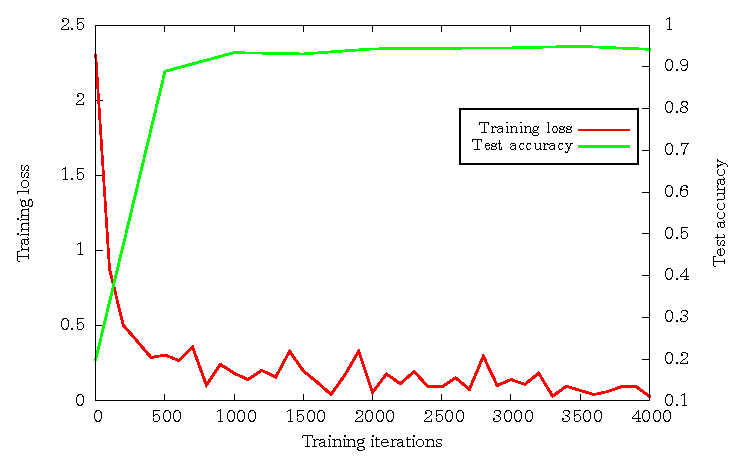
\includegraphics[scale=1.0]{fig/eps/result_train_test_graph.eps}
 \caption{損失関数の値と精度 }
\end{figure}
\end{frame}

%%%% ogata %%%%
\begin{frame}[fragile]\frametitle{誤差関数}
 \begin{block}{caffe}
 多クラス分類:ソフトマックス関数\\
 誤差関数:交差エントロピー
 \end{block}

 \begin{exampleblock}{事後分布}
  \begin{equation}
   p({\bf d}|{\bf x}) = \prod_{k=1}^{K}p(C_k|{\bf x})^{d_k}
  \end{equation}
 \end{exampleblock}

 \begin{itemize}
	\item ${\bf d}$ : 目標出力
	\item ${\bf x}$ : 入力
	\item $C_k$ : 正解クラスの組($k=1,...,K$)
 \end{itemize}

\end{frame}

\begin{frame}[fragile]\frametitle{誤差関数}

 \begin{exampleblock}{訓練データに対する{\bf w}の尤度}
  \begin{equation}
    L({\bf w})=\prod_{n=1}^{N}p({\bf x}_n|{\bf x}_n;{\bf
	w})=\prod_{n=1}^{N}\prod_{k=1}^{K}p(C_k|{\bf
	x})^{d_{nk}}=\prod_{n=1}^{N}\prod_{k=1}^{K}(y_k({\bf x};{\bf w}))^{d_{nk}}
  \end{equation}
 \end{exampleblock}

 \begin{itemize}
	\item 訓練データ : ${({\bf x}_n|{\bf d}_n)}(n=1,...,N)$
	\item {\bf w} : ネットワークのパラメータを成分に持つベクトル
 \end{itemize}

この尤度の対数とって符号を反転した次の式を誤差関数として用いる.

 \begin{exampleblock}{交差エントロピー}
  \begin{equation}
   E({\bf w})=-\sum^{N}_{n=1}\sum^{N}_{k=1}d_{nk}\log
  \end{equation}
 \end{exampleblock}

\end{frame}

%%%% Pythonを用いたキャラクター識別用プログラムの作成 %%%%
\begin{frame}\frametitle{Pythonを用いたキャラクター識別用プログラムの作成}
\begin{itemize}
  \item 前回までで独自のデータセットを用意して学習を行い,モデルを作成した.
  \item Caffeでは.caffemodelという形式で保存され,これとCNNがどのように構成されているのかを表す.prototxtファイルを用いてキャラクター識別用プログラムを作成した.
  \item これらを扱うためのCaffeが提供しているAPIと,\\画像を読み込んだり入力した画像に識別結果を書き込むためにOpenCVを用いた.
\end{itemize}
\end{frame}

%%%% Pythonを用いたキャラクター識別用プログラムの作成 %%%%
\begin{frame}[fragile]\frametitle{Pythonを用いたキャラクター識別用プログラムの作成}
まず.caffemodelと.prototxtを読み込む部分のプログラムを示す.

\begin{lstlisting}[basicstyle=\ttfamily\footnotesize, language=Python, frame=single, firstnumber=1, numbers=left, breaklines=true]
classifier = caffe.Classifier(
        'cifar10_full.prototxt',
        'cifar10_full_150717_iter_60000.caffemodel',
        mean=mean_array,
        raw_scale=255)
\end{lstlisting}
そして,入力画像からOpenCVで実装されているHaar-like特徴量から人の顔を抽出し,これをCaffeの識別器にかける.
\\この部分のプログラムを示す.

\begin{lstlisting}[basicstyle=\ttfamily\footnotesize, language=Python, frame=single, firstnumber=1, numbers=left, breaklines=true]
predictions = classifier.predict([image], oversample=False)
pred = np.argmax(predictions)
\end{lstlisting}

classifier.predict()で抽出された顔が各ラベルの人の顔である確率がリターンされる.
この値と関連付けられたキャラクター名をOpenCVのAPIを用いて入力画像に書き込む.
これをHaar-like特徴量から取得された顔の数だけ繰り返す.
\end{frame}


%%%% Caffeで識別 %%%%
\begin{frame}\frametitle{caffeを使った識別}
前回の発表で説明した識別器を用いて実際に識別してみる.

\begin{figure}[t]
 \begin{minipage}{0.45\hsize}
  \centering
  \text{ラブライブ!} \\
  \centering
  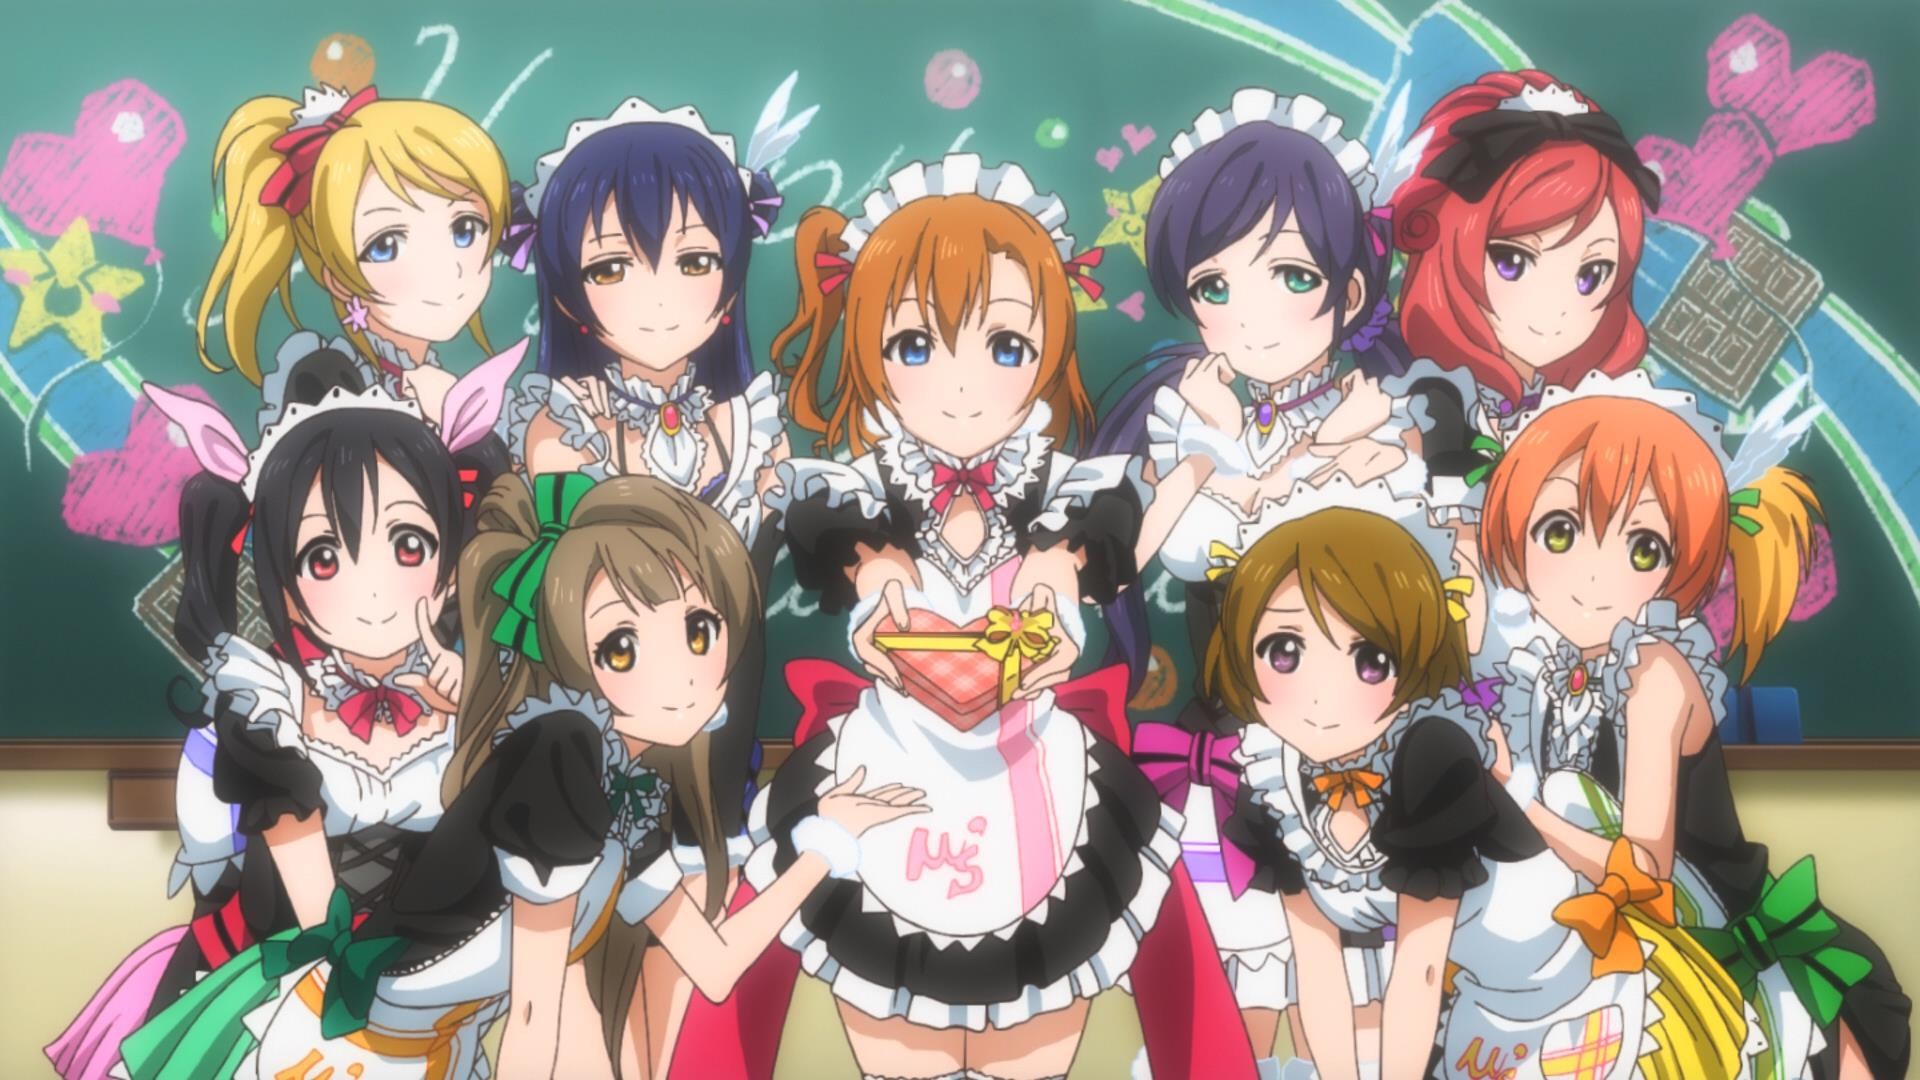
\includegraphics[width=50mm]{./fig/jpg/lovelive.jpg} \\
  \text{登録されている}
  \text{アニメキャラクターの画像}
 \end{minipage}
 \begin{minipage}{0.45\hsize}
  \centering
  \text{アイドルマスター} \\
  \centering
  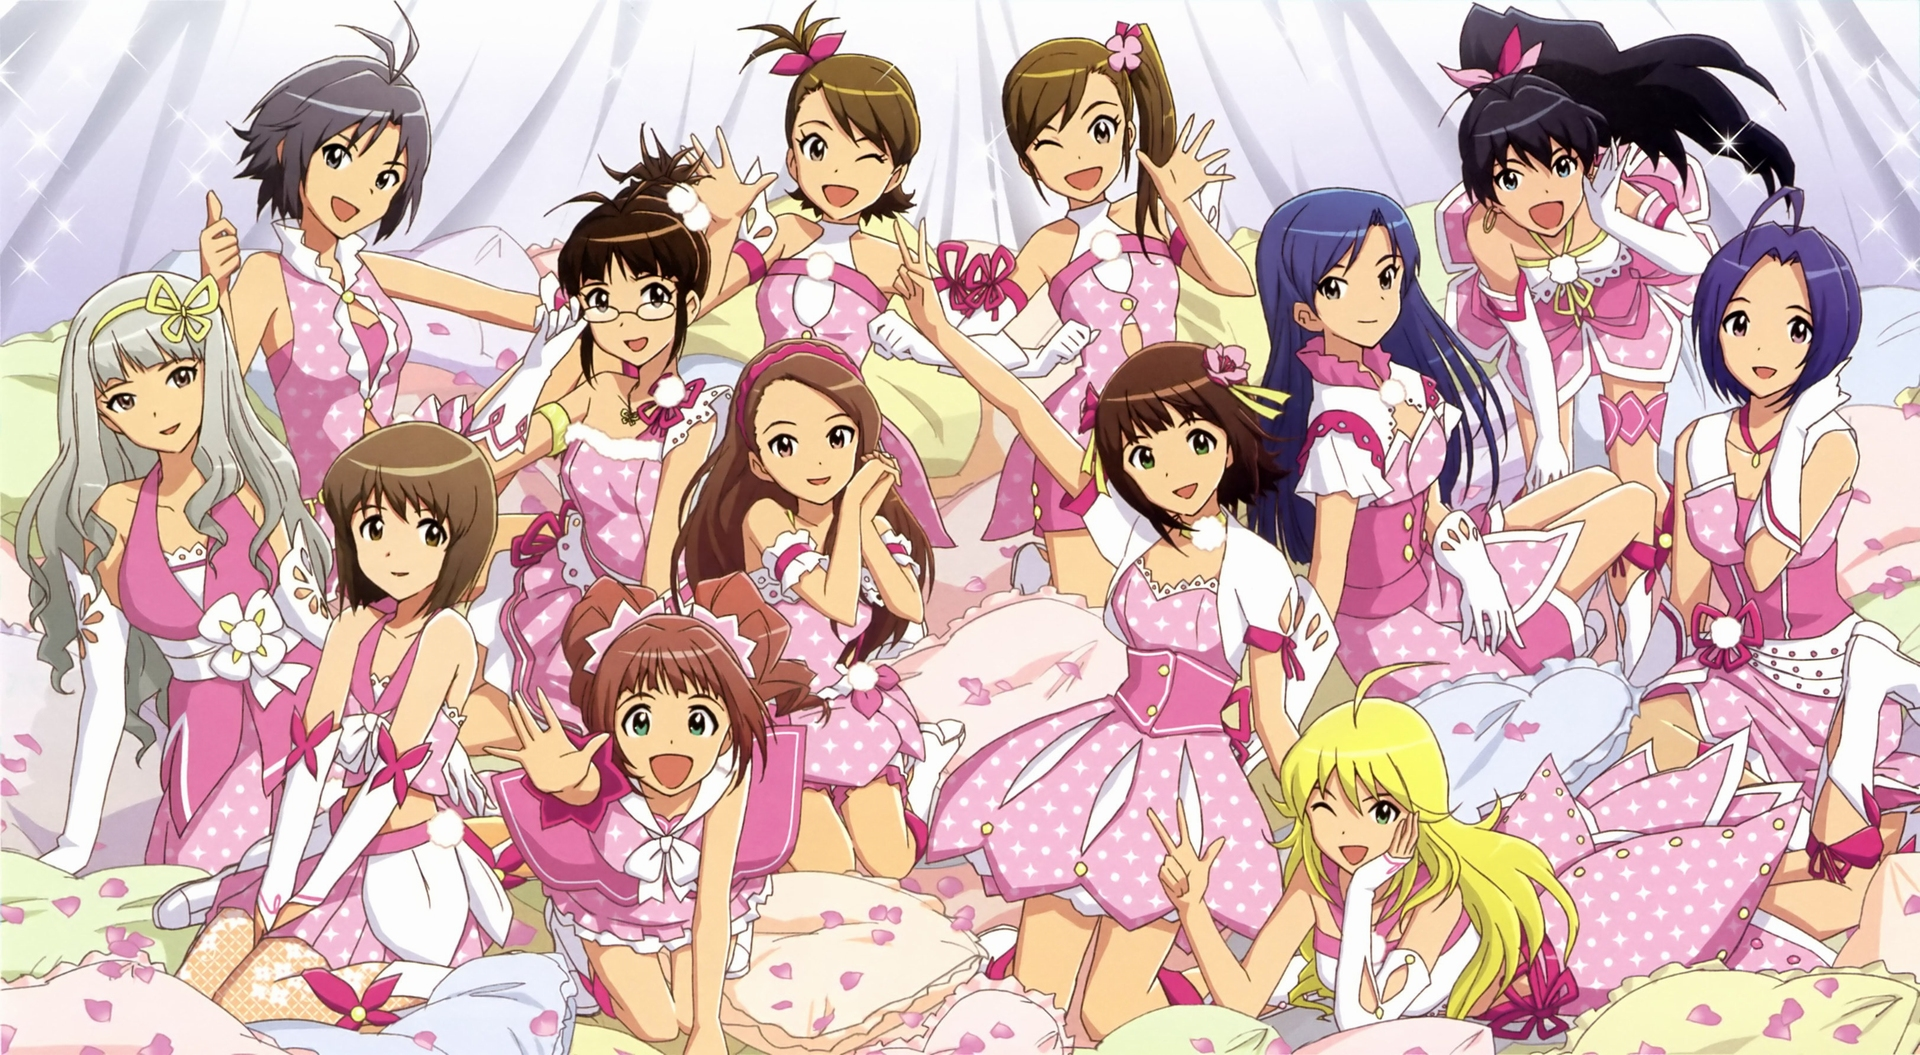
\includegraphics[width=50mm]{./fig/jpg/idolmaster.jpg}\\
  \text{登録されていない}
  \text{アニメキャラクターの画像}
 \end{minipage}
\end{figure}
\end{frame}

%%%% Caffeで識別結果1 %%%%
\begin{frame}\frametitle{caffeを使った識別結果}

\begin{figure}[t]
  \centering
  \text{ラブライブ!} \\
  \centering
  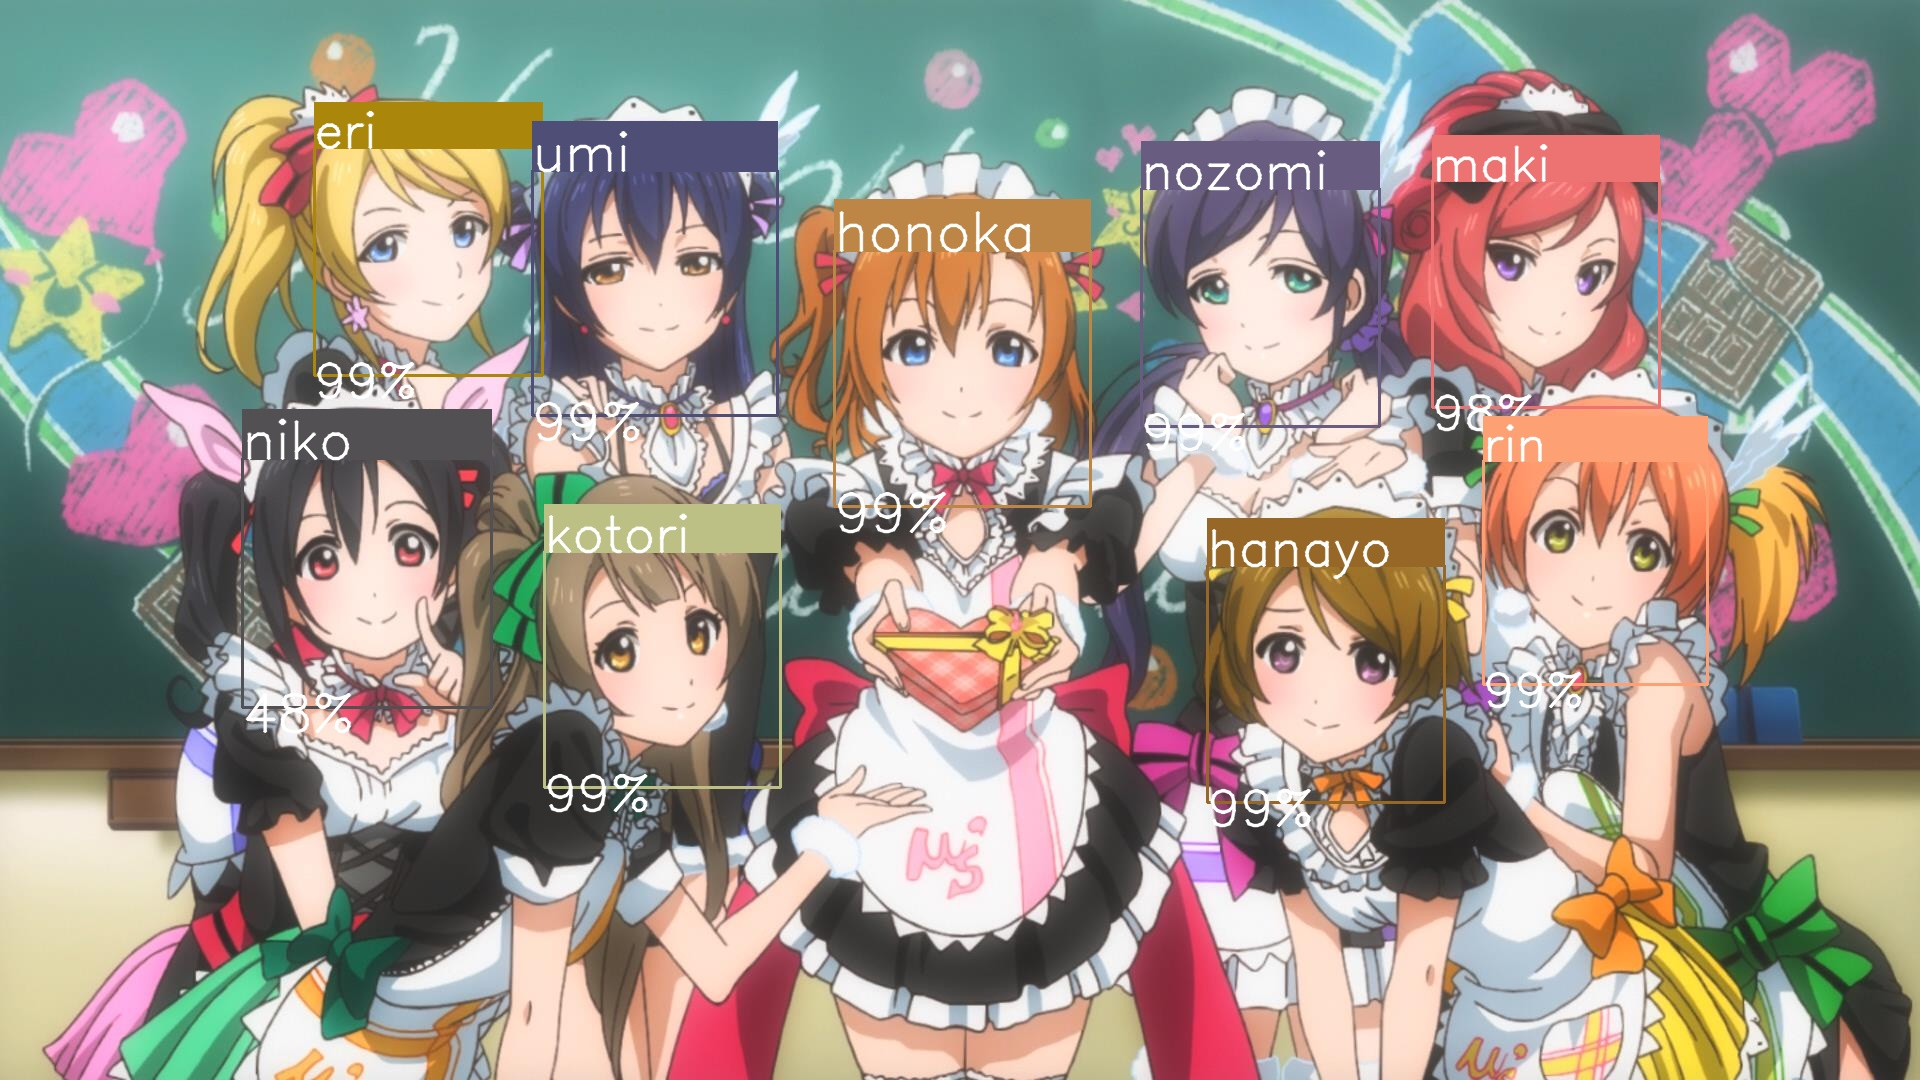
\includegraphics[width=100mm]{./fig/jpg/result_lovelive.jpg} \\
  \text{登録されている}
  \text{アニメキャラクターの画像}
\end{figure}
\end{frame}

%%%% Caffeで識別結果2 %%%%
\begin{frame}\frametitle{caffeを使った識別結果}

\begin{figure}[t]
  \centering
  \text{アイドルマスター} \\
  \centering
  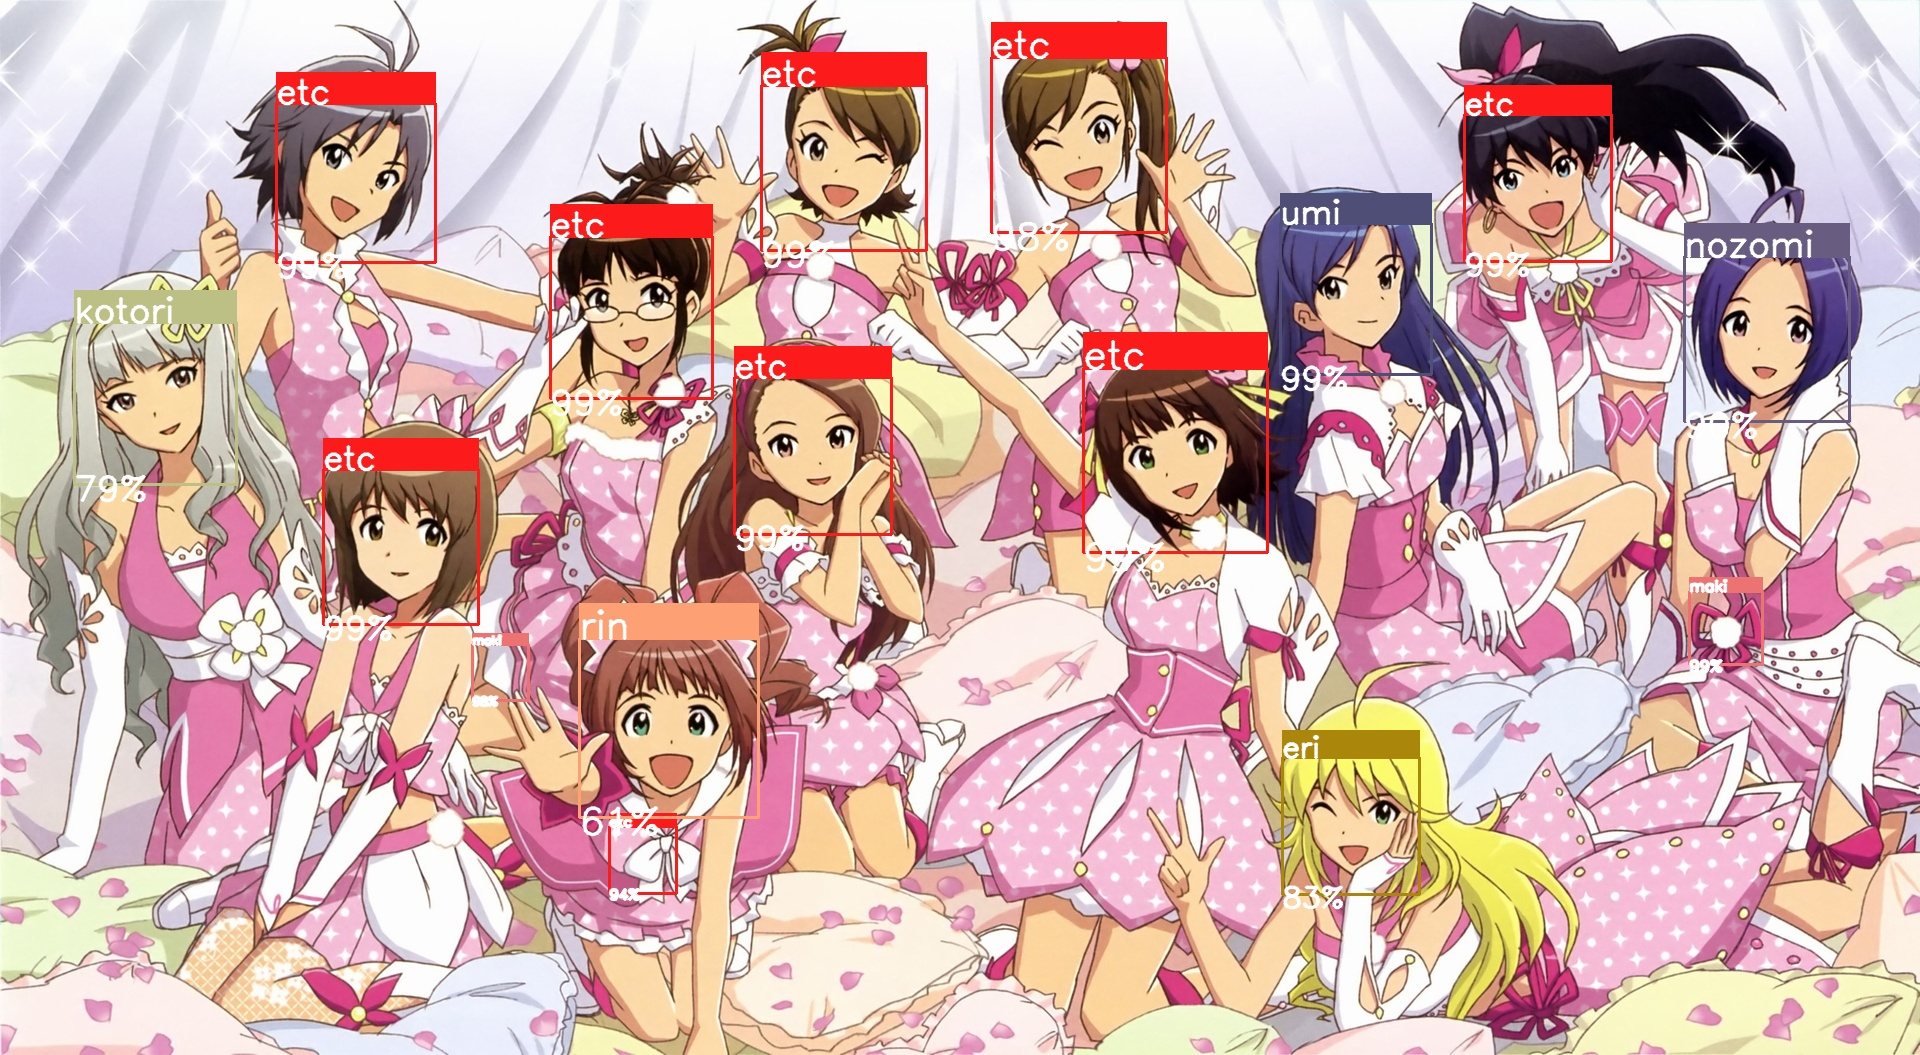
\includegraphics[width=100mm]{./fig/jpg/result_idolmaster.jpg} \\
  \text{登録されていない}
  \text{アニメキャラクターの画像}
\end{figure}
\end{frame}

%%%% Caffeで識別結果3 %%%%
\begin{frame}\frametitle{caffeを使った識別結果}

\begin{figure}[t]
  \centering
  \text{真のラベルとの比較} \\
  \centering
  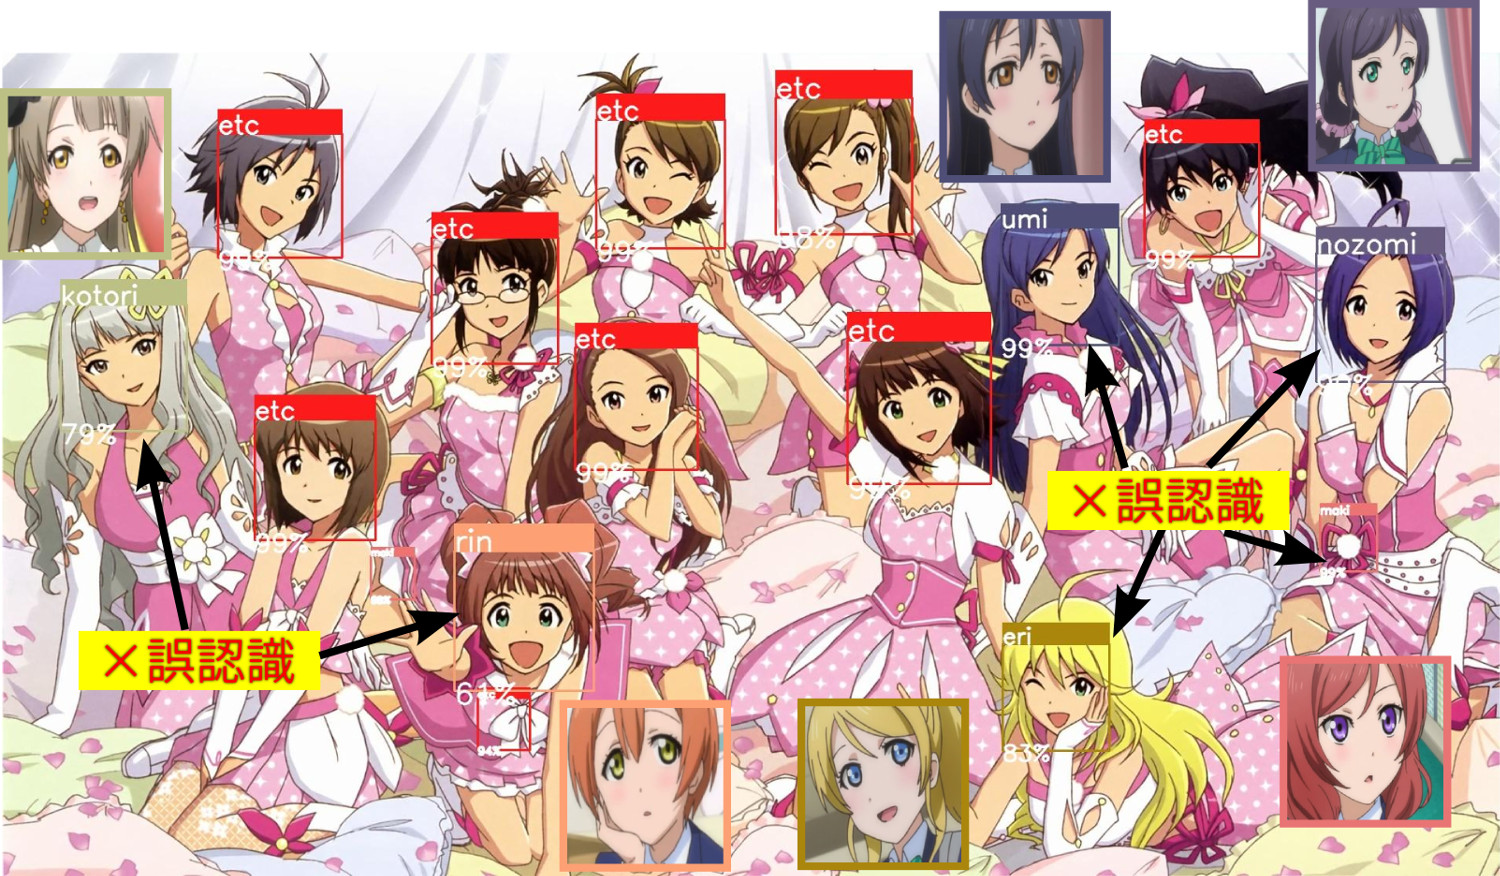
\includegraphics[width=100mm]{./fig/jpg/result_idol_compare.jpg} \\
  \text{登録されていない}
  \text{アニメキャラクターの画像}
\end{figure}
\end{frame}

%%%% 今後の課題 %%%%
\begin{frame}\frametitle{今後の課題}

\begin{block}{理論研究}
CNNの詳細な調査
\end{block}

\vspace{1cm}
\begin{exampleblock}{プログラミング}
学習画像を追加したり、パラメータを変更してみる
\end{exampleblock}
\end{frame}

% \begin{figure}[t]
%  \begin{minipage}{0.3\hsize}
%   \centering
%   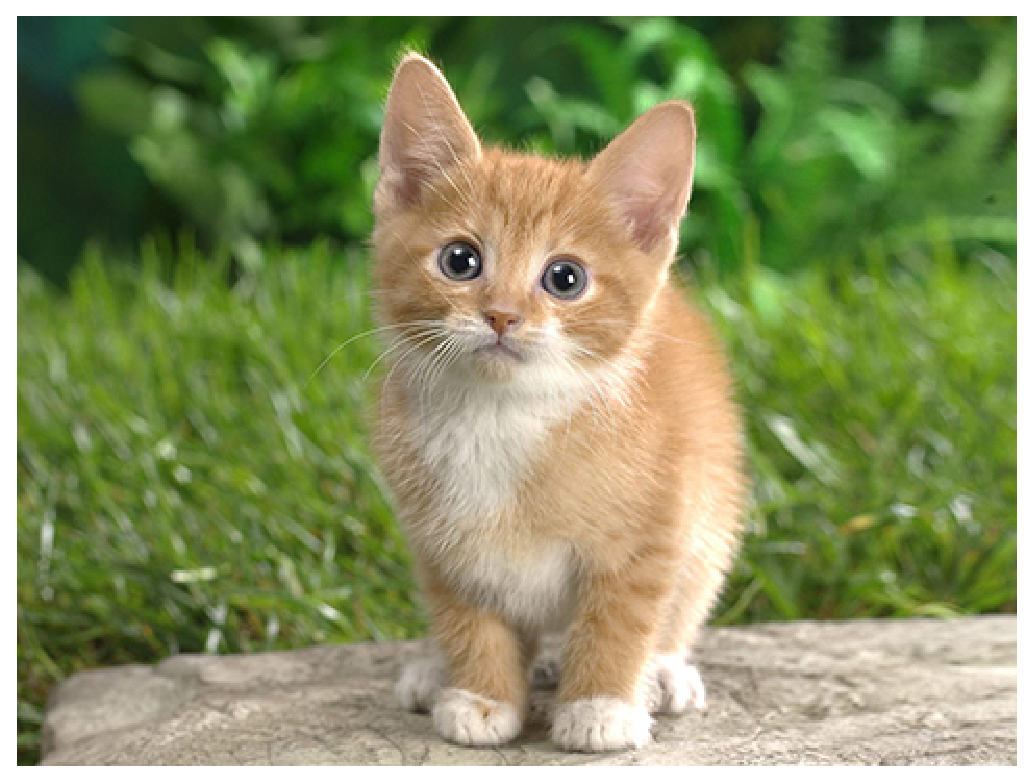
\includegraphics[width=30mm]{./figure/cat.eps}
%   \caption{cat.jpg}
%   \label{sample1}
%  \end{minipage}
%  \begin{minipage}{0.3\hsize}
%   \centering
%   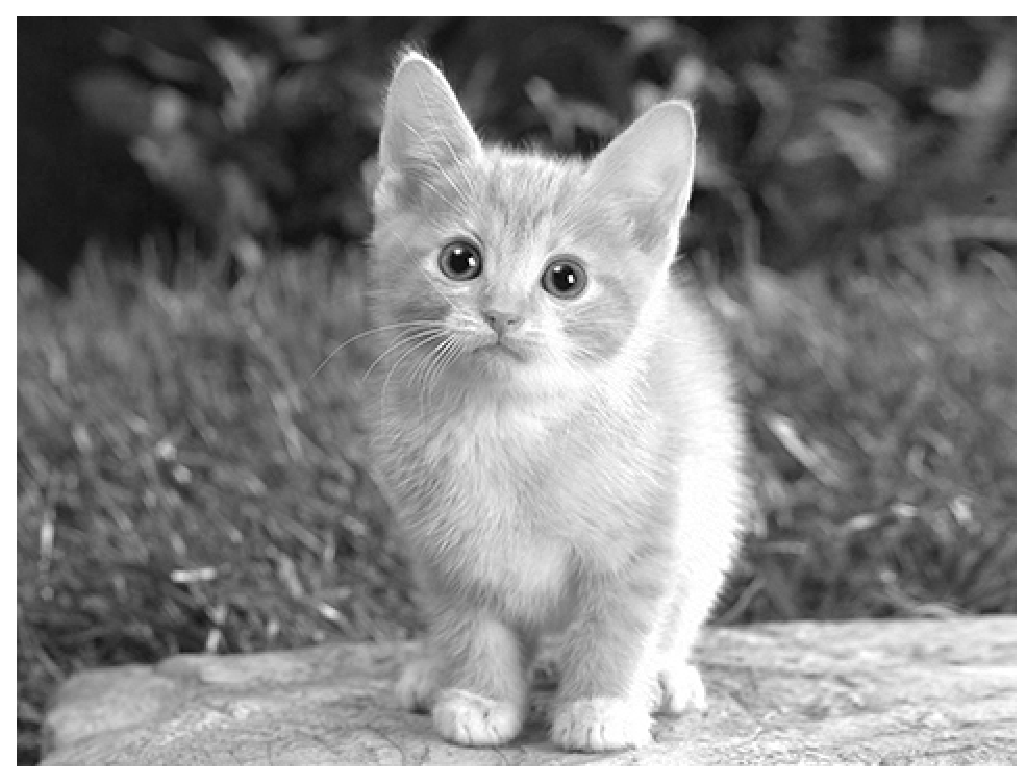
\includegraphics[width=30mm]{./figure/cat_gray.eps}
%   \caption{cat\_gray.jpg}
%   \label{sample2}
%  \end{minipage}
%  \begin{minipage}{0.3\hsize}
%   \centering
%   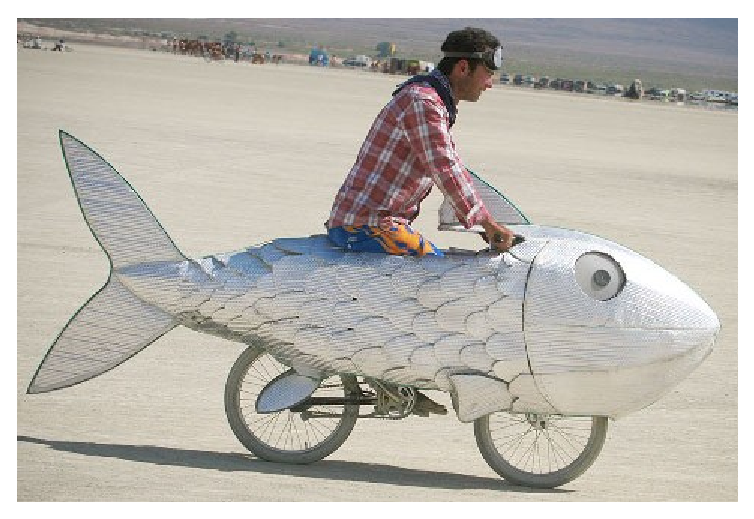
\includegraphics[width=30mm]{./figure/fish-bike.eps}
%   \caption{fish-bike.jpg}
%   \label{sample3}
%  \end{minipage}
% \end{figure}
% \begin{exampleblock}{実行環境}
% \begin{itemize}
%  \item Ubuntu 14.04 LTS
%  \item Intel core i5-4440 3.10GHz$\times$4
%  \item RAM 16GB
% \end{itemize}
% \end{exampleblock}
% \end{frame}


% \section{具体例}

% \begin{frame}\frametitle{定理環境の例}
% \begin{theorem}[Fermat]
% $a^{p-1} \equiv 1 \pmod{p}$
% \end{theorem}
% \pause
% \begin{theorem}[Wilson]
% \begin{equation}
% (p-1)! \equiv 1 \pmod{p}
% \end{equation}
% \end{theorem}
% \end{frame}

% \begin{frame}<1-2>\frametitle{オーバーレイ}
% \onslide*<1>{
% \Large{これは1枚目です}
% }
% \onslide*<2>{
% これは2枚目です
% \begin{theorem}[Euclid]
% There is no largest prime number.
% \end{theorem}
% }
% \end{frame}

% \begin{frame}\frametitle{色もつけれるよ}
%   {\color{red} red}(\alert{alert}),
%   {\color{blue} blue}(\structure{structure}),
%   {\color{green} green},
%   {\color{cyan} cyan},
%   {\color{magenta} magenta},
%   {\color{yellow} yellow},
%   {\color{black} black},
%   {\color{darkgray} darkgray},
%   {\color{gray} gray},
%   {\color{lightgray} lightgray},
%   {\color{orange} orange},
%   {\color{violet} violet},
%   {\color{purple} purple},
%   {\color{brown} brown},
% \end{frame}

% \begin{frame}\frametitle{いろんなブロック}
% \begin{block}{ブロック}
% これは普通のブロックです
% \end{block}

% \begin{alertblock}{警告ブロック}
% 警告!これは警告ブロックだ!
% \end{alertblock}

% \begin{exampleblock}{例ブロック}
% 例えば、こんなブロックです。
% \end{exampleblock}
% \end{frame}

% \begin{frame}<1-2>\frametitle{画像も貼れるよ}
% \onslide*<1>{
% このように画像を貼れるよ
% %\begin{figure}[htb]
% %\centering
% %\includegraphics[width=12cm,clip]{dummygraph.pdf}
% %\caption{$f(x)=e^{-\frac{x}{10}}\sin(x)$}
% %\end{figure}%
% }
% \onslide*<2>{
% 画像や表は各自用意してね
% %\begin{figure}[htb]
% %\centering
% %\includegraphics[width=8cm,clip]{sym4.pdf}
% %\caption{Cayley graph of $\mathfrak{S}_{4}$}
% %\end{figure}%
% }
% \end{frame}

% \begin{frame}\frametitle{まとめ}
% \LARGE{大事なのは中身です!}
% \end{frame}

% \begin{frame}\frametitle{}
% {\Large ありがとうございました}
% \end{frame}
% \appendix

\newcounter{finalframe}
\setcounter{finalframe}{\value{framenumber}}

% \begin{frame}[containsverbatim]\frametitle{dvipngの使い方(1)}
% \begin{block}{この様なファイルを用意する}
% \tiny{
% \begin{verbatim*}
% \documentclass[43pt]{jsarticle}
% \usepackage{amsmath}
% \usepackage{lmodern}
% \pagestyle{empty}
% \begin{document}
% \begin{equation*}
% \sum_{k=0}^{\infty} \frac{(2k)!}{2^{2k}(k!)^2} \frac{1}{2k+1}=\frac{\pi}{2}
% \end{equation*}
% \end{document}
% \end{verbatim*}
% }
% \end{block}
% \end{frame}

% \begin{frame}[containsverbatim]\frametitle{dvipngの使い方(2)}
% \begin{block}{使い方(コマンドライン)}
% \scriptsize{
% \begin{verbatim*}
% latex dvipng-sample.tex
% dvipng dvipng-sample.dvi -T tight -bd 1000
% \end{verbatim*}
% }
% \end{block}
% \end{frame}
\setcounter{framenumber}{\value{finalframe}}
\end{document}